\documentclass{article}

\usepackage{fancyhdr}
\usepackage[margin=2cm]{geometry}
\usepackage{graphicx}
\usepackage{graphics}
\usepackage{hyperref}
\usepackage{psfrag}
\usepackage{ifthen}
\usepackage{array}
\usepackage{longtable}
\usepackage{color}
\usepackage{tikz}
\usetikzlibrary{arrows.meta}
\usepackage{bm}
\usepackage{amsmath, amsfonts}
\usepackage[shortlabels]{enumitem}
\setcounter{secnumdepth}{0}
\newcommand{\N}{\mathbb{N}}
\newcommand{\R}{\mathbb{R}}

\begin{document}

\title{Homework Set \#1}
\author{Hayden Pott}
\date{4 April 2024}

\fancyhead{} % clear all header fields
\fancyhead[R]{Hayden Pott}
\fancyhead[L]{Homework Set \#1}
\renewcommand\headrulewidth{0pt}
\fancyfoot{} % clear all footer fields
\fancyfoot[C]{\thepage}

\pagestyle{fancy}
\maketitle

\begin{enumerate}[1.]

        \section{Lecture 1}
    \item Define the term ``alphabet''. Define the term ``language''. Explain the
        differences between these two concepts. \\
        ANSWER: \\
        Alphabet - A set of characters used by a language to form words \\
        Language - A set of words created from an alphabet and rules \\
        An alphabet contains characters while a language contains sequences
        of characters
    \item Given the language $S^*$ defined over the set $S = \{aa, b\}$ write
        down ALL words of length 4 contained in $S^*$ \\
        ANSWER: $\{aaaa, aabb, baab, bbaa, bbbb\}$
    \item Provide an English description of this language. Be as precise as
        possible. $L = \{b^{2N+1} \text{ for } N = 0,1,2,3,\dots\}$ \\
        ANSWER: All strings of b's with odd length greater or equal to 1
    \item Prove that ``abba'' is a word in $S^*$ given the underlying set $S =
        \{a, b, ab\}$. Does ``abba'' have a unique factorization? If not, show
        ALL possible ways of constructing ``abba'' from the factors of $S$.
        \begin{enumerate}[a)]
            \item ...
                ANSWER: ``abba'' can be constructed as $(ab)(b)(a)$
            \item Does ``abba'' have a unique factorisation? If not, show ALL
                possible ways of constructing ``abba'' from the factors of $S$.
                \\ 
                ANSWER: No, it can be written as $(ab)(b)(a)$ or $(a)(b)(b)(a)$
        \end{enumerate}

        \section{Lecture 2}
    \item Given the language ``all even length strings of b’s''
        \begin{enumerate}[a)]
            \item Define this language using the listing method we covered in
                Lecture 1 \\
                ANSWER: $S = \{\Lambda, bb, bbbb, bbbbbb, \dots\}$
            \item Define this language using the mathematical notation method we
                covered in Lecture 1. \\
                ANSWER: $L = \{b^{2N} \text{ for } N = 0, 1, 2, \dots\}$
            \item Define this language using the recursive definition method
                presented in this lecture. \\
                ANSWER:
                \begin{enumerate}[1)]
                    \item $\Lambda$ is a word in $L$
                    \item If $Q$ is any word in $L$, the $\text{CONCAT}(Q,$
                        ``$bb$''$)$ is also a word in $L$
                    \item $L$ contains only those words that can be generated from
                        Rules 1 and 2
                \end{enumerate}
        \end{enumerate}
    \item Provide a regular expression for ``all even length strings of b's'' \\
        ANSWER: $\bm{(bb)^*}$
    \item List all words of length 4 in Language((a+b)* a). Also, provide an
        English description of this language. \\
        ANSWER: $\{aaaa, aaba, abaa, abba, baaa, baba, bbaa, bbba\}$
    \item Generate a regular expression of ``all words over the alphabet $\Sigma
        = \{a, b\}$ that either begin with a and end with b OR begin with b and
        end in a.'' Thus, the first few shortest words in this language are
        ``ab'' ``ba'' ``aab'' ``baa'' ``abb'' ``bba'' ``aaab'' etc. So, if a
        word begins with a it must in end b, and if it begins with b it must end
        in a. \\
        ANSWER: $\bm{(a(a+b)^*b)+(b(a+b)^*a)}$

    \item Consider the language ``all words that can be constructed from the
        alphabet $\Sigma = \{a, b\}$ that contain exactly two b's.''
        \begin{enumerate}[a)]
            \item List the four shortest words in the language \\
                ANSWER: $\{bb, abb, bba, aabb\}$
            \item Generate a regular expression that for this language. \\
                ANSWER: $\bm{a^*bba^*}$
        \end{enumerate}
        \section{Lecture 3}
    \item Consider the language of ``all words over the alphabet $\Sigma = {a, b}$
        that both (a) end in `bb' and (b) contain only one instance of `bb'.''
        \begin{enumerate}[a)]
            \item List the seven shortest words in this language. \\
                ANSWER: $S = \{bb, abb, aabb, babb, aaabb\}$
            \item Construct a regular expression for this language.\\
                ANSWER: $\bm{a^*(baa^*)^*bb}$
        \end{enumerate}

    \item Using the formal definitions of both the syntax and semantics of
        regular expressions, construct the regular expression $\bm{(ab^* +
        ba^*)}$ and its associated language in a step-by-step manner from the
        definitions. Show all steps. See slide 7 for an example.
        \begin{itemize}
            \item $\bm{a}$ is a regular expression by Syntax Rule 1.1 and
                $\{a\}$ is its language by Semantic Rule 1.1

            \item $\bm{b}$ is a regular expression by Syntax Rule 1.1 and
                $\{b\}$ is its language by Semantic Rule 1.1

            \item $\bm{b^*}$ is a regular expression by Syntax Rule 2.3 and
                $\{\Lambda, b, bb, bbb, \dots\}$ is its language by Semantic
                Rule 2.3 [Closure of $\{b\}$ under concatenation]

            \item $\bm{ab^*}$ is a regular expression by Syntax Rule 2.1 and
                $\{a, ab, abb, abbb, \dots\}$ is its language by Semantic Rule
                2.1 [product set of $\{a\}$ and $\{\Lambda, b, bb, bbb,
                \dots\}$]

            \item $\bm{a^*}$ is a regular expression by Syntax Rule 2.3 and
                $\{\Lambda, a, aa, aaa, \dots\}$ is its language by Semantic
                Rule 2.3 [Closure of $\{a\}$ under concatenation]

            \item $\bm{ba^*}$ is a regular expression by Syntax Rule 2.1 and
                $\{b, ba, baa, baaa, \dots\}$ is its language by Semantic Rule
                2.1 [product set of $\{b\}$ and $\{\Lambda, a, aa, aaa,
                \dots\}$]

            \item $\bm{ab^* + ba^*}$ is a regular expression by Syntax Rule 2.2 and
                $\{\Lambda, a, b, ab, ba, aab, baa, aaab, baaa, \dots\}$ is its language by Semantic Rule
                2.2 [union of \{a, ab, abb, abbb, \dots\} and \{b, ba, baa, baaa, \dots\}]

            \item $\bm{(ab^* + ba^*)}$ is a regular expression by Syntax Rule
                2.0 and $\{\Lambda, a, b, ab, ba, aab, baa, aaab, baaa, \dots\}$
                continues to be its associated language
        \end{itemize}

    \item Refer to the Finite Automaton given on Slides 11 and 12.
        \begin{enumerate}[a)]
            \item Trace the path taken by the string ``bbbab'' through the
                machine \\
                ANSWER: $X \to b \to X \to b \to X \to b \to X \to a \to Y \to b \to Y$
            \item Is the word ``bbbab'' accepted by the machine? \\
                ANSWER: Yes, we end on a final state.
        \end{enumerate}

    \item Does every regular expression define a language? \\
        ANSWER: Yes, for any regular expression, we can use it to produce
        strings using the rules defined in the expression, therefore creating a
        language by definition.
    \item Does every finite automaton define a language? \\
        ANSWER: Yes, for any finite automaton, we can use it to produce strings
        (or validate from a set of strings), therefore creating a
        language by definition.

        \section{Lecture 4}
    \item Consider the language of ``all (and only) the words over the alphabet
        $\Sigma = \{a, b\}$ that have a $b$ as their second letter.''
        \begin{enumerate}[a)]
            \item Draw a finite automaton for this language. \\
                ANSWER: \\
                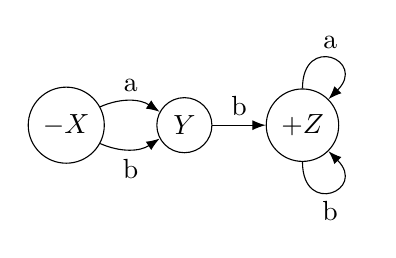
\begin{tikzpicture}[node distance={15mm}, main/.style = {draw, circle}] 
                    \node[main] (X) {$-X$}; 
                    \node[main] (Y) [right of=X] {$Y$};
                    \node[main] (Z) [right of=Y] {$+Z$};
                    \path[-Latex, bend left=10mm] (X) edge node[above] {a} (Y);
                    \path[-Latex, bend right=10mm] (X) edge node[below] {b} (Y);
                    \path[-Latex] (Y) edge node[above] {b} (Z);
                    \path[-Latex] (Z) edge [out=90,in=45,looseness=5] node[above] {a} (Z);
                    \path[-Latex] (Z) edge [out=270,in=315,looseness=5] node[below] {b} (Z);
                    %\path[->] (1) edge node[above] {a} (2);
                    %\path[->] (1) edge [out=90,in=180,looseness=10] node[above] {a} (1);
                \end{tikzpicture} 

            \item Construct a regular expression for this language. \\
                ANSWER: $\bm{(a+b)b(a+b)^*}$
        \end{enumerate}

    \item Build a finite automaton that accepts: Language ($\bm{(a (a+b)^* b) +
        (b (a+b)^* a)}$) \\
        ANSWER: \\
        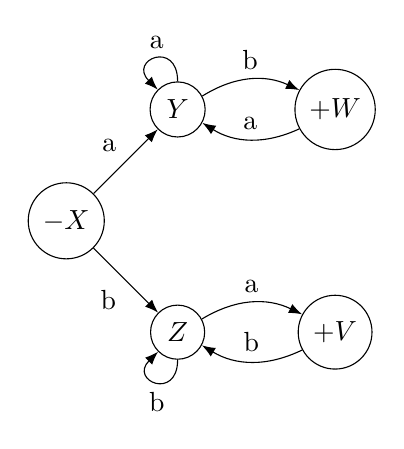
\begin{tikzpicture}[node distance={20mm}, main/.style = {draw, circle}] 
            \node[main] (X) {$-X$}; 
            \node[main] (Y) [above right of=X] {$Y$};
            \node[main] (Z) [below right of=X] {$Z$};
            \node[main] (W) [right of=Y] {$+W$};
            \node[main] (V) [right of=Z] {$+V$};

            \path[-Latex] (X) edge node[above left] {a} (Y);
            \path[-Latex] (X) edge node[below left] {b} (Z);

            \path[-Latex] (Y) edge [out=90,in=135,looseness=5] node[above] {a} (Y);
            \path[-Latex, bend left=10mm] (W) edge node[above] {a} (Y);
            \path[-Latex, bend left=10mm] (Y) edge node[above] {b} (W);

            \path[-Latex] (Z) edge [out=270,in=225,looseness=5] node[below] {b} (Z);
            \path[-Latex, bend left=10mm] (V) edge node[above] {b} (Z);
            \path[-Latex, bend left=10mm] (Z) edge node[above] {a} (V);

            %\path[->] (1) edge node[above] {a} (2);
            %\path[->] (1) edge [out=90,in=180,looseness=10] node[above] {a} (1);
        \end{tikzpicture}

    \item Consider the language consisting of all (and only) the words over the
        alphabet $\{a, b\}$ that end in ``ba''.
        \begin{enumerate}[a)]
            \item Draw a finite automaton for this language. \\
                ANSWER: \\
                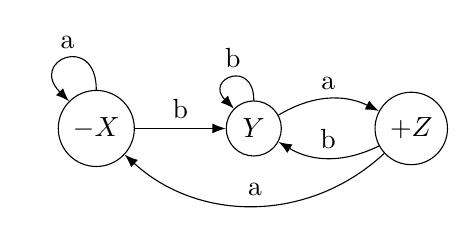
\begin{tikzpicture}[node distance={20mm}, main/.style = {draw, circle}] 
                    \node[main] (X) {$-X$}; 
                    \node[main] (Y) [right of=X] {$Y$};
                    \node[main] (Z) [right of=Y] {$+Z$};

                    \path[-Latex] (X) edge node[above] {b} (Y);
                    \path[-Latex] (X) edge [out=90,in=135,looseness=5] node[above] {a} (X);

                    \path[-Latex] (Y) edge [out=90,in=135,looseness=5] node[above] {b} (Y);

                    %\path[-Latex] (Y) edge node[above] {a} (Z);
                    %\path[-Latex] (Y) edge node[above] {a} (Z);

                    \path[-Latex, bend left=10mm] (Y) edge node[above] {a} (Z);
                    \path[-Latex, bend left=10mm] (Z) edge node[above] {b} (Y);
                    \path[-Latex, bend left=15mm] (Z) edge node[above] {a} (X);

                    %\path[->] (1) edge node[above] {a} (2);
                    %\path[->] (1) edge [out=90,in=180,looseness=10] node[above] {a} (1);
                \end{tikzpicture}
            \item Construct a regular expression for this language. \\
                ANSWER: $\bm{(a+b)^*ba}$
        \end{enumerate}

    \item Draw a finite automaton for the language consisting of all (and only)
        the words over the alphabet $\{a, b\}$ that do NOT end in ``ba''. \\
        ANSWER: \\
        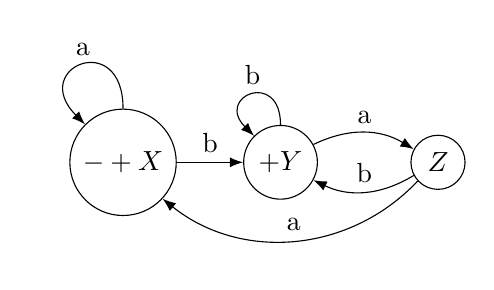
\begin{tikzpicture}[node distance={20mm}, main/.style = {draw, circle}] 
            \node[main] (X) {$-+X$}; 
            \node[main] (Y) [right of=X] {$+Y$};
            \node[main] (Z) [right of=Y] {$Z$};

            \path[-Latex] (X) edge node[above] {b} (Y);
            \path[-Latex] (X) edge [out=90,in=135,looseness=5] node[above] {a} (X);

            \path[-Latex] (Y) edge [out=90,in=135,looseness=5] node[above] {b} (Y);

            %\path[-Latex] (Y) edge node[above] {a} (Z);
            %\path[-Latex] (Y) edge node[above] {a} (Z);

            \path[-Latex, bend left=10mm] (Y) edge node[above] {a} (Z);
            \path[-Latex, bend left=10mm] (Z) edge node[above] {b} (Y);
            \path[-Latex, bend left=15mm] (Z) edge node[above] {a} (X);

            %\path[->] (1) edge node[above] {a} (2);
            %\path[->] (1) edge [out=90,in=180,looseness=10] node[above] {a} (1);
        \end{tikzpicture}

    \item Draw a finite automation with exactly three states that accepts
        Language($\bm{(a+b)^*}$) \\
        ANSWER: \\
        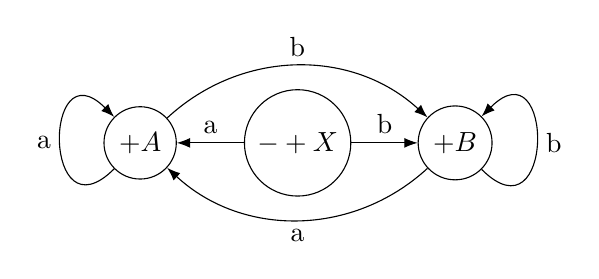
\begin{tikzpicture}[node distance={20mm}, main/.style = {draw, circle}] 
            \node[main] (X) {$-+X$}; 
            \node[main] (A) [left of=X] {$+A$};
            \node[main] (B) [right of=X] {$+B$};

            \path[-Latex] (X) edge node[above] {a} (A);
            \path[-Latex] (X) edge node[above] {b} (B);

            \path[-Latex] (A) edge [out=225,in=135,looseness=5] node[left] {a} (A);
            \path[-Latex] (B) edge [out=-45,in=45,looseness=5] node[right] {b} (B);

            \path[-Latex, bend left=15mm] (B) edge node[below] {a} (A);
            \path[-Latex, bend left=15mm] (A) edge node[above] {b} (B);

            %\path[->] (1) edge node[above] {a} (2);
            %\path[->] (1) edge [out=90,in=180,looseness=10] node[above] {a} (1);
        \end{tikzpicture}

\end{enumerate}

\end{document}
